% !TEX root = main.tex

\section{LLVM framework quick start}


\begin{frame}{Simulating a LLVM driver manually}
	\noindent\hspace{-1.2cm}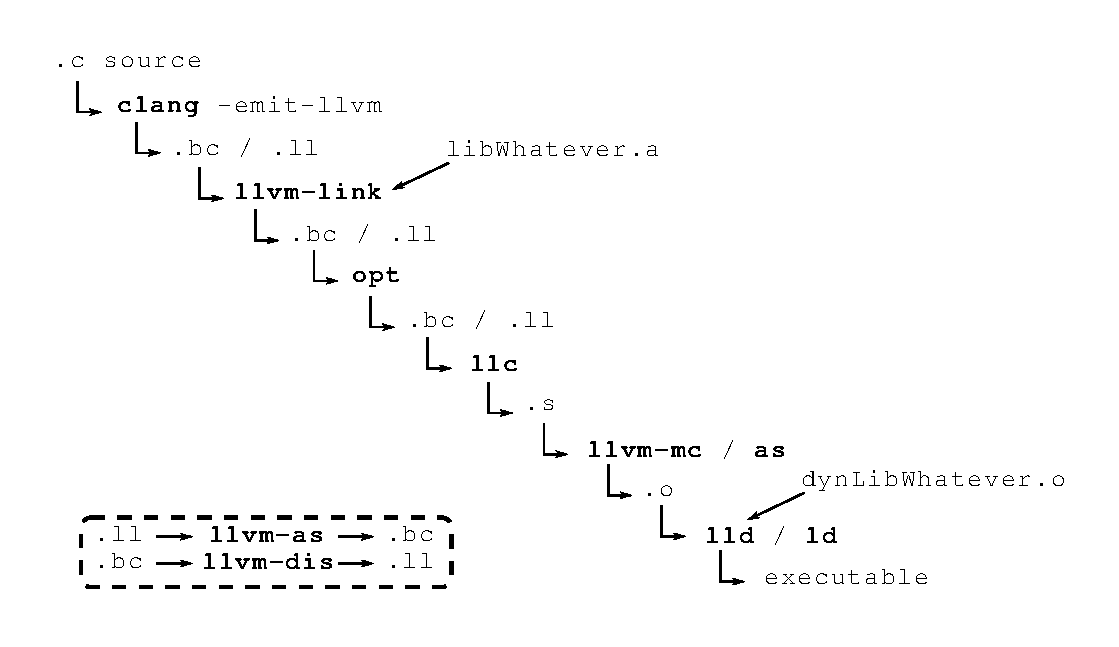
\includegraphics[width=13cm]{img/toolchain}
\end{frame}


\begin{frame}{Writing a LLVM pass}
	There are a lot of tutorials available:
	\vfill
	\begin{itemize}
		\item Official developer guide\\ \href{http://llvm.org/docs/WritingAnLLVMPass.html}{\url{llvm.org/docs/WritingAnLLVMPass}}
		\vfill
		\item Out-of-source pass\\ \href{https://github.com/quarkslab/llvm-dev-meeting-tutorial-2015}{\url{github.com/quarkslab/llvm-dev-meeting-tutorial-2015}}
	\end{itemize}
	\vfill
	We will follow the first one, with a few adjustments.
\end{frame}


\begin{frame}{Building LLVM}
\begin{center}
To test your pass you need a \alert{Debug+Assertions} build of LLVM.\\
\bigskip
This build needs to be \alert{kept separated} from normal Release builds (it's very slow!)\\
\bigskip
The best way to get such a LLVM build is to \alert{make it yourself}!
\end{center}
\end{frame}


\begin{frame}{Building LLVM}
\begin{itemize}
\item Detailed instructions: \url{https://llvm.org/docs/GettingStarted.html}
\end{itemize}
\bigskip
\begin{description}
\item[Problem 1] With the \alert{default options}, a finished build takes\\\alert{25 GB of disk space}
\item[Problem 2] A standard build with the GNU toolchain uses \alert{a lot of RAM} ($\approx$16 GB or more with a modern 4 core CPU!) especially when linking
\end{description}
\bigskip
We need to customize the build process a bit...
\end{frame}


\begin{frame}{Building LLVM}
\begin{itemize}
\item The build flags I like to use:\\
\smallskip\texttt{\small-GNinja \\
-DLLVM\_ENABLE\_PROJECTS='clang' \\
-DLLVM\_INSTALL\_UTILS=ON \\
\textbf{-DLLVM\_BUILD\_LLVM\_DYLIB=ON \\
-DLLVM\_LINK\_LLVM\_DYLIB=ON} \\
-DLLVM\_OPTIMIZED\_TABLEGEN=ON \\
-DLLVM\_INCLUDE\_EXAMPLES=OFF \\
-DCMAKE\_INSTALL\_PREFIX=/opt/llvm-9.0-d \\
\textbf{-DLLVM\_USE\_LINKER=lld \\
-DCMAKE\_C\_COMPILER=clang-9 \\
-DCMAKE\_CXX\_COMPILER=clang++-9} \\
}
\item Building with LLVM itself solves the RAM usage problem!
\item Using \alert{shared libraries} drops the disk usage to \alert{10 GB}.\\
{\footnotesize The build products alone will still take 20 GB of disk space...}
\end{itemize}
\end{frame}


\begin{frame}{Testing}
LLVM has an internal testing infrastructure\footnote{\url{http://llvm.org/docs/TestingGuide.html}}.
Please use it.
\\
\begin{description}
	\item[llvm-lit] LLVM Integrated Tester
\end{description}
\begin{enumerate}
	\item Forge a proper LLVM-IR input file (.ll) for your test case
	\item Instrument it with \texttt{lit} script comments
	\item Run \texttt{lit} on your test
		\begin{itemize}
			\item \texttt{llvm-lit ~/llvm/test/myTests/singleTest.ll}\\ run a single test
			\item \texttt{llvm-lit ~/llvm/test/myTests}\\ run the test suite (folder)
		\end{itemize}
	\item Run \texttt{lit} on the LLVM test suite (regression testing)
\end{enumerate}
\vfill
To submit a bug report to LLVM developers you will be asked to write a \texttt{lit} test case that highlights the bug.
\end{frame}
